\documentclass[11pt,]{article}
\usepackage[]{mathpazo}
\usepackage{amssymb,amsmath}
\usepackage{ifxetex,ifluatex}
\usepackage{fixltx2e} % provides \textsubscript
\ifnum 0\ifxetex 1\fi\ifluatex 1\fi=0 % if pdftex
  \usepackage[T1]{fontenc}
  \usepackage[utf8]{inputenc}
\else % if luatex or xelatex
  \ifxetex
    \usepackage{mathspec}
  \else
    \usepackage{fontspec}
  \fi
  \defaultfontfeatures{Ligatures=TeX,Scale=MatchLowercase}
\fi
% use upquote if available, for straight quotes in verbatim environments
\IfFileExists{upquote.sty}{\usepackage{upquote}}{}
% use microtype if available
\IfFileExists{microtype.sty}{%
\usepackage{microtype}
\UseMicrotypeSet[protrusion]{basicmath} % disable protrusion for tt fonts
}{}
\usepackage[margin=1in]{geometry}
\usepackage{hyperref}
\hypersetup{unicode=true,
            pdfborder={0 0 0},
            breaklinks=true}
\urlstyle{same}  % don't use monospace font for urls
\usepackage{natbib}
\bibliographystyle{apsr}
\usepackage{graphicx,grffile}
\makeatletter
\def\maxwidth{\ifdim\Gin@nat@width>\linewidth\linewidth\else\Gin@nat@width\fi}
\def\maxheight{\ifdim\Gin@nat@height>\textheight\textheight\else\Gin@nat@height\fi}
\makeatother
% Scale images if necessary, so that they will not overflow the page
% margins by default, and it is still possible to overwrite the defaults
% using explicit options in \includegraphics[width, height, ...]{}
\setkeys{Gin}{width=\maxwidth,height=\maxheight,keepaspectratio}
\IfFileExists{parskip.sty}{%
\usepackage{parskip}
}{% else
\setlength{\parindent}{0pt}
\setlength{\parskip}{6pt plus 2pt minus 1pt}
}
\setlength{\emergencystretch}{3em}  % prevent overfull lines
\providecommand{\tightlist}{%
  \setlength{\itemsep}{0pt}\setlength{\parskip}{0pt}}
\setcounter{secnumdepth}{0}
% Redefines (sub)paragraphs to behave more like sections
\ifx\paragraph\undefined\else
\let\oldparagraph\paragraph
\renewcommand{\paragraph}[1]{\oldparagraph{#1}\mbox{}}
\fi
\ifx\subparagraph\undefined\else
\let\oldsubparagraph\subparagraph
\renewcommand{\subparagraph}[1]{\oldsubparagraph{#1}\mbox{}}
\fi

%%% Use protect on footnotes to avoid problems with footnotes in titles
\let\rmarkdownfootnote\footnote%
\def\footnote{\protect\rmarkdownfootnote}

%%% Change title format to be more compact
\usepackage{titling}

% Create subtitle command for use in maketitle
\newcommand{\subtitle}[1]{
  \posttitle{
    \begin{center}\large#1\end{center}
    }
}

\setlength{\droptitle}{-2em}
  \title{}
  \pretitle{\vspace{\droptitle}}
  \posttitle{}
  \author{true}
  \preauthor{\centering\large\emph}
  \postauthor{\par}
  \predate{\centering\large\emph}
  \postdate{\par}
  \date{Y}


\begin{document}

\section{Parameters for Ebola}\label{parameters-for-ebola}

Culled from literature.

First read in and clean up the data from Health Map. Since these data
are at national level, we will also aggregate the WHO data at country
level. HealthMap collects and curates data on the cumulative number of
cases (C) and deaths (D) stratified by status (suspected, SC/SD, or
confirmed CC/CD). For data from the WHO, the case status could be
confirmed, probable or suspected. The final clinical outcome
(alive/dead) for each case is also recorded. In comparing the two data
sets, we sum across all four categories in Healthmap and derive
incidence data from cumulative data.

ProMED data is similarly stratfied and we will sum across the categories
of suspected and confirmed cases for ProMED.

\includegraphics{figures/weekly_incid_viz-1.pdf}

\subsection{Correlation between the incidence
data}\label{correlation-between-the-incidence-data}

\includegraphics{figures/incid_corrplot-1.pdf}

\subsection{Estimating Reproduction number from WHO and Healthmap
Data}\label{estimating-reproduction-number-from-who-and-healthmap-data}

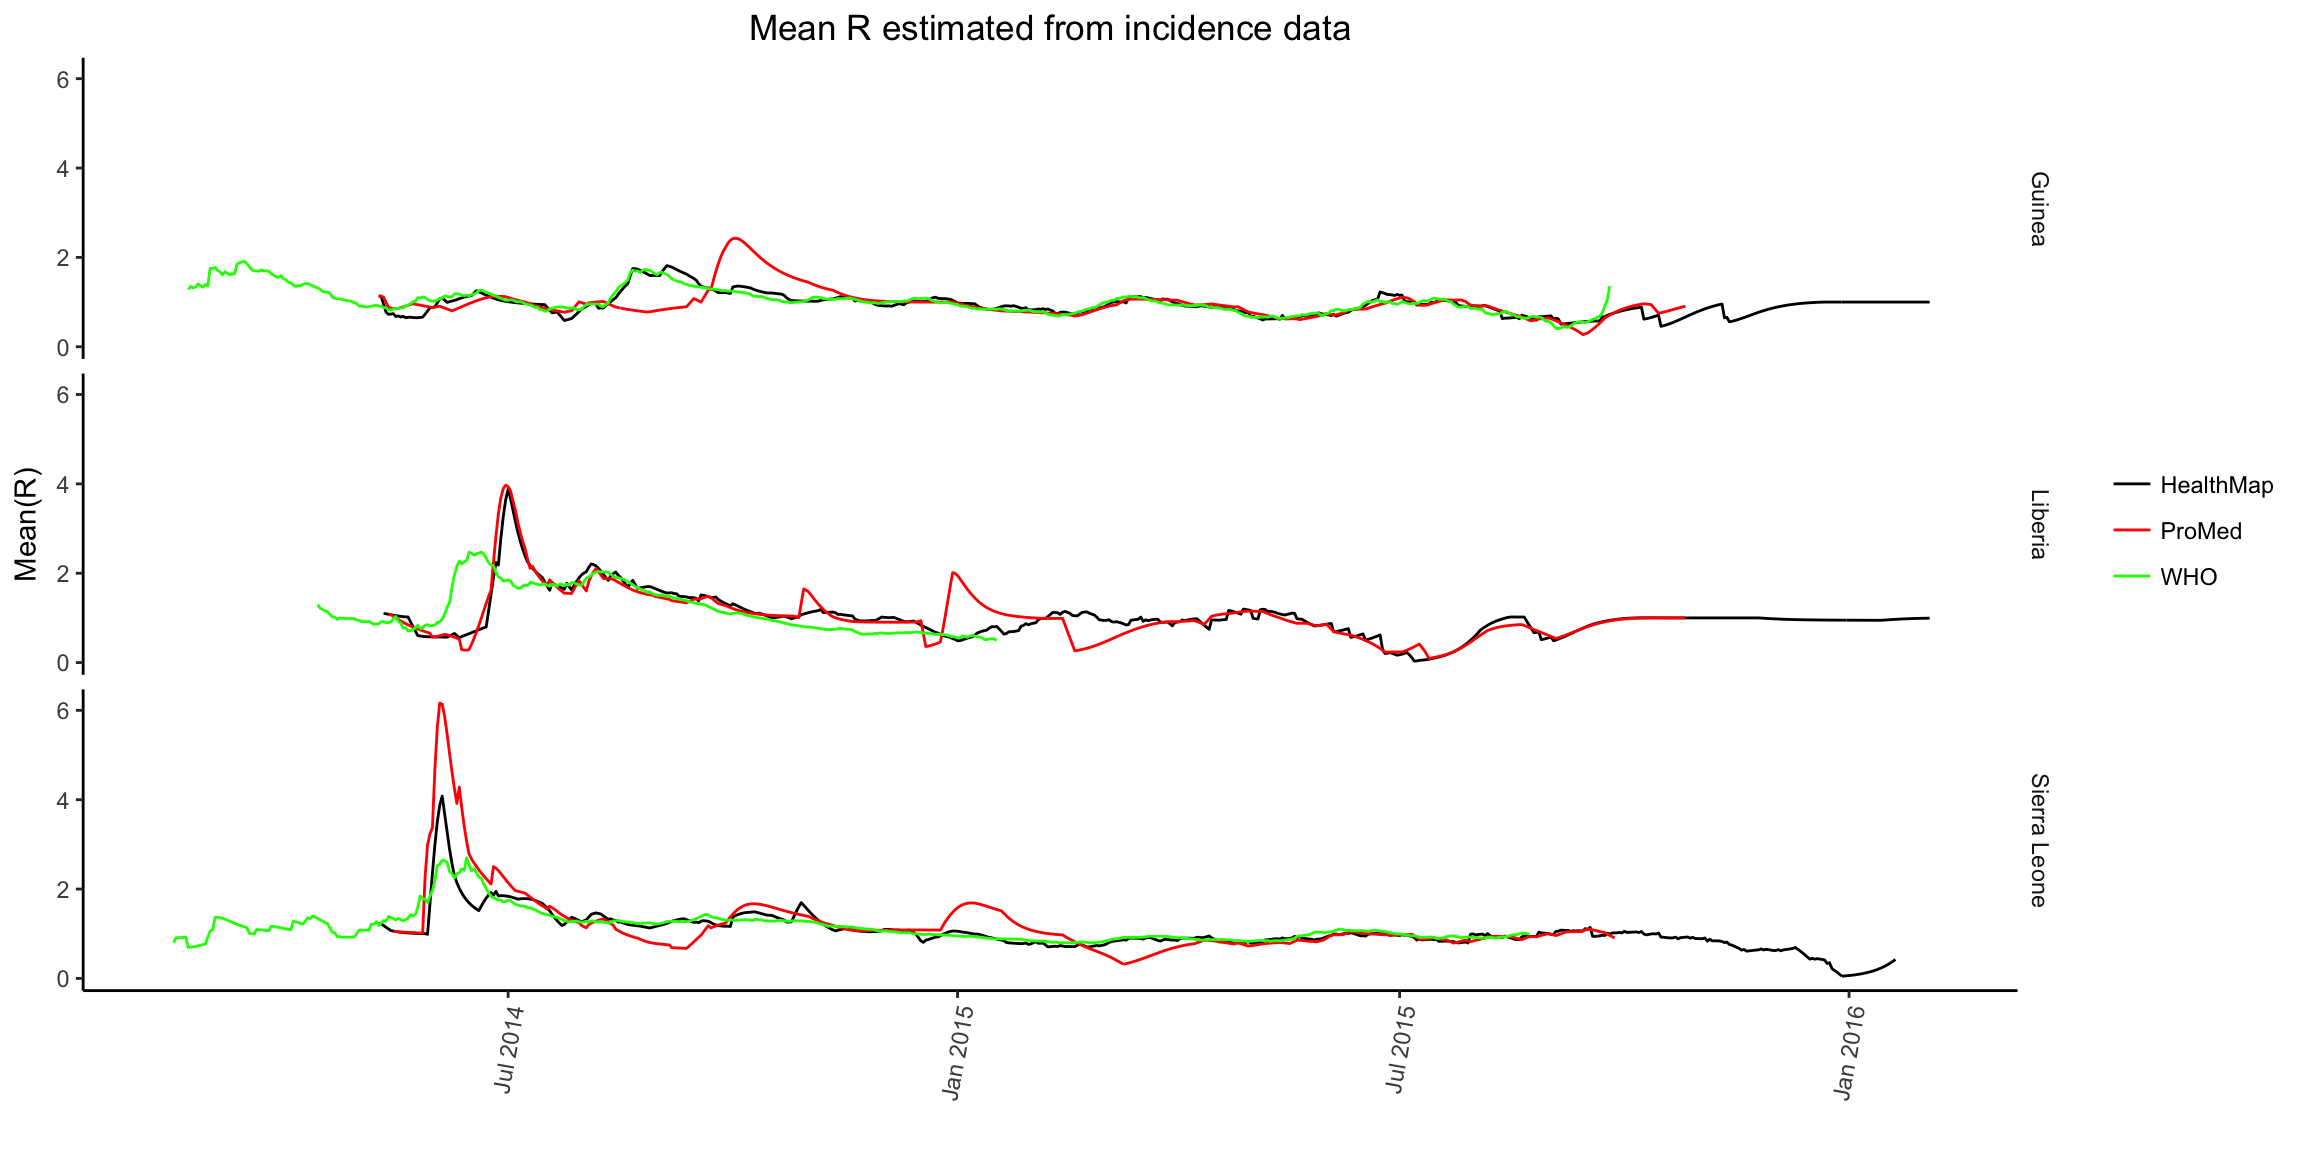
\includegraphics{figures/who_vs_hm_vs_pm-1.pdf}

The graphs show that the estimates from the three different sources
closely track each other. Here's another way to visualise this.

\includegraphics{figures/hm_who-1.pdf}

\includegraphics{figures/pm_who-1.pdf}

\includegraphics{figures/pm_hm-1.pdf} As the above graphs indicates,
estimates of the reproduction number from ProMed, HealthMap and WHO data
are highly correlated (correlation coefficient = 0.76, 95\% CI = (0.74,
0.78)).

\includegraphics{figures/R_corrplot-1.pdf}


\end{document}
